\documentclass[11pt,letterpaper]{article}
\usepackage[utf8]{inputenc}
\usepackage[T1]{fontenc}
\usepackage{mathptmx}
\usepackage[letterpaper,left=1.25in,right=1.25in,top=1.2in,bottom=1.2in,headheight=14pt]{geometry}
\usepackage{microtype}
\usepackage{amsmath,amssymb,amsthm,mathtools,bm}
\usepackage{graphicx,booktabs,array,multirow}
\usepackage{xcolor}
\usepackage{enumitem}
\usepackage[labelfont=bf,labelsep=colon,font=small,skip=4pt]{caption}
\usepackage{algorithm}
\usepackage{algpseudocode}
\usepackage{fancyhdr}
\usepackage{titlesec}
\usepackage[authoryear,round]{natbib}
\definecolor{linkcol}{HTML}{2B3A8F}
\usepackage[colorlinks=true,linkcolor=linkcol,citecolor=linkcol,urlcolor=linkcol]{hyperref}
\usepackage[capitalise,noabbrev]{cleveref}

\pagestyle{fancy}\fancyhf{}
\lhead{\small Preprint.}
\cfoot{\small\thepage}
\renewcommand{\headrulewidth}{0.5pt}
\setlength{\parskip}{4pt plus 1pt}\setlength{\parindent}{0pt}
\titleformat{\section}{\large\bfseries}{\thesection}{0.8em}{}
\titleformat{\subsection}{\normalsize\bfseries}{\thesubsection}{0.8em}{}
\titleformat{\subsubsection}{\normalsize\bfseries\itshape}{\thesubsubsection}{0.8em}{}
\titlespacing*{\section}{0pt}{16pt}{6pt}\titlespacing*{\subsection}{0pt}{12pt}{4pt}
\setlist{itemsep=1pt,topsep=3pt}

\theoremstyle{plain}
\newtheorem{proposition}{Proposition}
\newtheorem{theorem}{Theorem}
\newtheorem{corollary}{Corollary}
\newtheorem{lemma}{Lemma}
\theoremstyle{definition}
\newtheorem{definition}{Definition}
\theoremstyle{remark}
\newtheorem{remark}{Remark}
\crefname{proposition}{Proposition}{Propositions}

\newcommand{\Z}{\mathbb{Z}}
\newcommand{\E}{\mathbb{E}}
\newcommand{\Var}{\mathrm{Var}}
\newcommand{\Lam}{\Lambda_N}
\newcommand{\TV}{\mathrm{TV}}
\newcommand{\unlike}{\mathcal{U}}
\newcommand{\Tb}{T_{\mathrm b}}
\newcommand{\Tc}{T_{\mathrm c}}
\newcommand{\Hdel}{\Delta H}
\newcommand{\Hpair}{\Delta H^{\mathrm{pair}}}
\newcommand{\Ind}{\mathbf{1}}
\newcommand{\EoneConfigs}{13\,824}
\newcommand{\EoneAdj}{512}
\newcommand{\EoneNonadj}{13\,312}
\newcommand{\EoneDisp}{35}
\newcommand{\EoneMismatch}{0}
\newcommand{\EtwoMaxTVcorrect}{3.9\times10^{-12}}
\newcommand{\EtwoMaxStatRes}{1.2\times10^{-16}}
\newcommand{\EtwoPairMin}{0.07}
\newcommand{\EtwoPairMax}{0.46}
\newcommand{\EtwoNNMin}{0.10}
\newcommand{\EtwoNNMax}{0.77}
\newcommand{\EthreeAdjHundred}{0.00041}
\newcommand{\EthreeAdjDiffMaxHundred}{0.00027}
\newcommand{\EthreeEquivOK}{yes}
\newcommand{\EthreeBareAcross}{6}
\newcommand{\EthreeBareWithin}{4}
\newcommand{\EthreeSeedAcross}{1}
\newcommand{\EthreeSeedWithin}{1}
\newcommand{\EthreeSpeedup}{144}
\newcommand{\EthreeJit}{0.74}
\newcommand{\EthreePy}{106}
\newcommand{\EfourSmallRatio}{4.2}
\newcommand{\EfourPredThirtyTwo}{0.0034}
\newcommand{\EfourSeThirtyTwo}{0.0031}
\newcommand{\EfourCountLargeSig}{1}
\newcommand{\EfourCountLarge}{9}
\newcommand{\EfourHundredZ}{+0.4}
\newcommand{\EfourMaxAbsZ}{28.7}
\newcommand{\EfourSmallN}{28.7}
\newcommand{\EfiveCentralIn}{16}
\newcommand{\EfiveCentralTot}{18}
\newcommand{\EfiveExtremeIn}{0}
\newcommand{\EfiveExtremeTot}{9}
\newcommand{\EfiveCentralInC}{14}
\newcommand{\EfiveExtremeInC}{0}
\newcommand{\EfiveExtBiasMin}{-0.29}
\newcommand{\EfiveExtBiasMax}{-0.17}
\newcommand{\EfiveExtZMin}{3.3}
\newcommand{\EfiveCenZMax}{4.1}
\newcommand{\EfiveCenZGtTwo}{5}
\newcommand{\EfiveCenTot}{18}
\newcommand{\EfiveCIWidthMin}{0.10}
\newcommand{\EfiveCIWidthMax}{0.60}
\newcommand{\EfiveCenBiasMax}{0.19}
\newcommand{\EfiveSdMin}{0.09}
\newcommand{\EfiveSdMax}{0.30}
\newcommand{\EfiveMeanAtFiveHundredthXXXII}{1.80}
\newcommand{\EfiveMeanAtFiveHundredthLXIV}{1.81}
\newcommand{\EfiveMeanAtFiveHundredthC}{1.81}
\newcommand{\EfiveTbAtFiveHundredth}{2.03}
\newcommand{\EsixZMax}{1.5}
\newcommand{\EfiveSymMin}{0.02}
\newcommand{\EfiveSymMax}{0.18}
\newcommand{\EfiveR}{8}
\newcommand{\EfiveBurn}{500}
\newcommand{\EfiveSample}{300}
\newcommand{\EfiveGridStep}{0.05}
\newcommand{\EfiveNT}{31}
\newcommand{\EbFiveHundredth}{2.032}
\newcommand{\EbTenth}{2.188}
\newcommand{\EbFifth}{2.261}
\newcommand{\EbThree}{2.269}
\newcommand{\EbHalf}{2.2692}
\newcommand{\EbDevTwoTenths}{0.0077}
\newcommand{\EbDevThreeTenths}{0.0003}
\newcommand{\EbRelTwoTenths}{0.3}
\newcommand{\EsixMaxAbsDev}{0.45}
\newcommand{\EsixMaxOver}{2.447}
\newcommand{\EsixMinDev}{-0.45}
\newcommand{\EsixMaxDev}{+0.18}
\newcommand{\EsixAsym}{0.24}
\newcommand{\EeightPerSpread}{1.6\times10^{-13}}
\newcommand{\EeightNonSpread}{26.6}
\newcommand{\EeightNonMin}{38.5}
\newcommand{\EeightNonMax}{65.1}
\newcommand{\EeightNonRel}{56}
\newcommand{\EeightPer}{32.81}
\newcommand{\EnineaRatioMin}{0.18}
\newcommand{\EnineaRatioMax}{1.35}
\newcommand{\EnineaRatioMedian}{0.56}
\newcommand{\EnineaBelowHalf}{4}
\newcommand{\EnineaCases}{11}
\newcommand{\EnineaOffMax}{2.3}
\newcommand{\EnineaOffGtOne}{3}
\newcommand{\EnineaTotalSweeps}{40\,000}
\newcommand{\EninebTauMax}{3797}
\newcommand{\EninebTauMedian}{28}
\newcommand{\EninebRuns}{432}


\setlength{\emergencystretch}{2em}

\title{\textbf{When Does a Monte Carlo Variance Peak Locate a Transition?}}
\begin{document}
\begin{center}
{\LARGE\bfseries When Does a Monte Carlo Variance Peak Locate a Transition?\\[4pt]
\Large Exact Exchange Sampling and Finite-Size Bias\\ in a Kawasaki--Ising Model of Segregation\par}
\vspace{1.4em}
{\bfseries\color{linkcol}\large Juan Fernando Casta\~no}\\[0.4em]
{\small New York University \quad $\cdot$ \quad \href{mailto:jfc9577@nyu.edu}{jfc9577@nyu.edu}}\par
\vspace{1.2em}
\end{center}
\begin{center}\textbf{Abstract}\end{center}
\vspace{-0.4em}
\begin{quote}\smallMonte Carlo output is only evidence about a phase transition if two things hold: the Markov chain samples the distribution we intend, and the observable we read off identifies the transition we intend. We examine both for the two-dimensional Ising lattice gas at fixed composition under pair-exchange (Kawasaki-type) Metropolis dynamics, used as a lattice model of residential segregation. First, we derive the exact exchange energy, which differs from the sum of two single-flip energies by $4J$ when the exchanged sites are neighbours, and prove that the resulting kernel is reversible, irreducible and aperiodic with the canonical law as its unique stationary distribution. Dropping the adjacency term breaks detailed balance by exactly $e^{\pm4\beta J}$; with uniform random-pair proposals the one-step perturbation is at most $4N^{-2}(1-e^{-4\beta J})$. A small one-step perturbation does not by itself bound the stationary one: on tori small enough to solve exactly the stationary law moves by $\EtwoPairMin$--$\EtwoNNMax$ in total variation, and at production sizes the mean-energy shift is a few per cent at $N=8,16$ and not detectable with our replication at $N\ge32$. Second, we compare the energy-variance peak, a common estimate of a transition or demixing temperature, with the exact fixed-composition coexistence curve obtained from Onsager and Yang. Over eight replicates, the single-run estimate has a standard deviation of $\EfiveSdMin$--$\EfiveSdMax$, larger than the whole composition dependence of the exact curve over $0.2\le f\le0.8$ ($\EbDevTwoTenths$, or $\EbRelTwoTenths\%$). At dilute compositions it lies $0.17$--$0.29$ below the exact curve. A long equilibrium reference shows that the standard 300-sweep sampling window is shorter than the energy autocorrelation time in the worst cases, but this does not account for the dilute offset, which persists in the equilibrium reference and is consistent with finite-size droplet formation. Tables, figures and the numbers in them are generated from stored raw output by the accompanying code.
\end{quote}
\vspace{0.4em}

\section{Introduction}
A Monte Carlo simulation produces numbers, and it is tempting to read them as measurements. A curve with a peak is read as a transition, and the temperature of the peak as the transition temperature. That reading needs two things to be true. The Markov chain has to sample the distribution we intend, and the observable we extract has to identify the physical quantity we intend. A simulation does not become trustworthy because it runs, equilibrates and produces a plausible-looking figure.

We check both conditions on a system where exact references exist for each. The system is the two-dimensional Ising lattice gas at fixed composition, evolved by pair-exchange Metropolis moves that conserve the number of each type. It is also a minimal statistical-physics model of residential segregation, in which a ``social temperature'' sets the balance between preference for like neighbours and tolerance of mixing \citep{schelling1971,vinkovic2006,stauffer2007,dallasta2008,gauvin2009}. In that literature a transition or demixing temperature is often read off simulation output. For this model we can say what the right answers are: the canonical law can be computed exactly on small tori, and the fixed-composition coexistence temperature is known in closed form from the work of Onsager and Yang \citep{onsager1944,yang1952}. That makes it possible to ask how far a standard simulation procedure is from them, and why.

\paragraph{Question 1: does the sampler target the canonical law?}
Exchanging two unlike spins is the same as flipping both. If the two sites are not neighbours the energy change is the sum of the two single-flip changes. If they are neighbours, the bond between them is unchanged by the exchange but is counted twice by that sum, and the exact change is the sum plus $4J$ (\cref{prop:delta}). The correction touches only a fraction $O(N^{-2})$ of uniformly random pair proposals, so it is small, and the interesting question is whether it matters statistically. A one-step perturbation of order $N^{-2}$ does not by itself imply a stationary-distribution perturbation of the same order; that depends on how fast the chain mixes. We therefore answer by proof where we can (detailed balance, irreducibility, a bound on the one-step perturbation), by exact stationary laws on tori small enough to solve, and by replicated simulation at production sizes. This is the foundation for the second question, whose conclusions are only meaningful if the chain is correct.

\paragraph{Question 2: given a correct sampler, does the variance peak locate the transition?}
A common estimate of a transition temperature is the location of the maximum of the energy variance over a temperature grid. At $f=1/2$ this is tied to the critical point. At other compositions the relevant reference is the fixed-composition coexistence (binodal) temperature $\Tb(f)$, and there is no divergence to locate: a finite system at fixed composition passes from a homogeneous state to coexistence through droplet formation, and this is rounded and displaced by finite-size effects \citep{binder1987,biskup2002}. So whether the variance peak tracks $\Tb(f)$ is a finite-size question rather than an identity. The exact curve is also nearly flat, with $\Tb(0.2)=\EbFifth$ against $\Tc=\EbHalf$, which means that a composition dependence of a few tenths in a simulated peak inside $0.2\le f\le0.8$ cannot be a property of the transition. Settling this requires the exact reference, replicate runs and a comparison with the resolution of the estimator, and it requires knowing whether the sampling window is long enough: the energy autocorrelation time can exceed the 300-sweep window of the protocol we study.

\paragraph{What we find.} The corrected exchange kernel has the canonical law as its unique stationary distribution, and we prove it. The version without the adjacency term has a stationary law far from canonical on small tori, but the effect on mean energy fades with lattice size under random-pair proposals and we cannot detect it for $N\ge32$ with the replication we could afford. The variance peak is noisy, its single-run scatter is larger than the entire composition dependence of the exact curve in the central range, and at dilute compositions it sits systematically below the exact curve. The long equilibrium reference does not remove that offset.

\paragraph{Contributions.} We do not propose a new model or algorithm. Our contributions are the following:
\begin{enumerate}[leftmargin=2em]
\item \textbf{Exact exchange energetics and detailed balance.} We derive the exact exchange energy (\cref{prop:delta}) and its attainable values (\cref{cor:values}), and prove that the exchange kernel is reversible, irreducible and aperiodic with the canonical law as unique stationary distribution (\cref{thm:correct}). Verified exhaustively on all $\EoneConfigs$ local configurations of a $6\times6$ torus with no mismatch.
\item \textbf{Local kernel error versus stationary law.} Without the adjacency term, detailed balance fails by exactly $e^{\pm4\beta J}$ (\cref{prop:flux}) and the one-step perturbation is at most $4N^{-2}(1-e^{-4\beta J})$ (\cref{prop:footprint}). We separate this local statement from the stationary one: exact stationary laws on tori of up to $8008$ states are $\EtwoPairMin$--$\EtwoPairMax$ (random-pair) and $\EtwoNNMin$--$\EtwoNNMax$ (nearest-neighbour proposals) from canonical in total variation, against $\EtwoMaxTVcorrect$ for the corrected kernel; replicated simulation gives a mean-energy shift of $5.5$--$6.3\%$ at $N=8$ and $1.0$--$2.2\%$ at $N=16$, and none we can detect at $N\ge32$.
\item \textbf{The variance peak against the exact binodal.} Over $\EfiveR$ replicates, three sizes and nine compositions, the single-run standard deviation is $\EfiveSdMin$--$\EfiveSdMax$; the central-range location is within $\EfiveCenBiasMax$ of the exact curve but too coarse to resolve its composition dependence; at dilute compositions it lies $0.17$--$0.29$ below it, with $|z|\ge\EfiveExtZMin$ in all nine cells.
\item \textbf{Equilibration and finite-size effects.} In long traces the 300-sweep window is shorter than the energy autocorrelation time in the worst cells and biases the variance. An equilibrium reference run shows the dilute offset is not a protocol artefact; it is consistent with finite-size droplet formation, though we do not test the scaling (\cref{sec:results-equil}).
\item \textbf{A reproducible pipeline.} Code, raw output and a generator for every table and figure (\cref{app:repro}).
\end{enumerate}
Contributions 1 and 2 give the computational foundation and quantify how a local kernel error propagates to equilibrium; contributions 3 and 4 ask whether the standard estimator locates the transition.

\paragraph{Organisation.} \Cref{sec:related} gives background. \Cref{sec:theory} treats the exchange kernel and \cref{sec:thermo} the thermodynamic reference and the estimator. \Cref{sec:protocol} describes the experiments. \Cref{sec:results} examines the sampler, \cref{sec:results-demix} the estimator, and \cref{sec:discussion} states what the study does and does not establish.

\section{Background}\label{sec:related}
\paragraph{Segregation models as spin systems.}
\citet{schelling1971} showed that mild local preferences produce macroscopic segregation. The connection to spin systems has been developed by \citet{vinkovic2006}, who cast Schelling dynamics as a lattice gas with an energy, by \citet{stauffer2007}, who relate it to the Ising model, by \citet{dallasta2008}, who study phase behaviour of Schelling dynamics in one and two dimensions, and by \citet{gauvin2009}, who map the phase diagram of a model with vacancies. In these works the structure of the model is read off Monte Carlo output. We study a minimal member of the family: two types, no vacancies, ferromagnetic nearest-neighbour coupling and conserved composition. Our subject is the sampler and an estimator applied to its output, not a new sociological model.

\paragraph{Exchange dynamics and kernel perturbations.}
The Metropolis rule \citep{metropolis1953} and Kawasaki's conserved-order-parameter dynamics \citep{kawasaki1966} are standard \citep{newman1999}. A sampler is correct when its kernel is reversible with respect to the target and irreducible \citep{levin2009}. How far a perturbed kernel moves the stationary law is controlled by the mixing properties of the unperturbed chain and is typically bounded as $\|\tilde\pi-\pi\|\le K(P)\|\tilde P-P\|$ \citep{mitrophanov2005}. We use this only qualitatively and measure the shift exactly where the state space permits.

\paragraph{Coexistence, droplets and finite-size effects.}
The square-lattice Ising model has an exact critical temperature \citep{onsager1944} and spontaneous magnetisation \citep{yang1952}, and through the lattice-gas correspondence these fix the coexistence curve in the composition--temperature plane \citep{rowlinson1982}. In a finite system at fixed composition the passage from a homogeneous state to coexistence is rounded and goes through droplet formation, displaced from the thermodynamic binodal \citep{binder1987,biskup2002}. A maximum of an energy-fluctuation estimate is therefore an estimator whose relation to the binodal has to be established, not assumed.

\section{The Exchange Kernel: Exact Energetics and Detailed Balance}
\label{sec:theory}
This section settles the first question. We define the chain, derive the exact exchange energy, prove that the resulting kernel has the canonical law as its stationary distribution, and then ask what happens to the stationary law when the adjacency term is dropped.

\subsection{The segregation Ising model}
Let $N\ge 3$ and $\Lam=(\Z/N\Z)^2$ be the $N\times N$ discrete torus, with edge set $\mathcal E=\{\{x,x+e_1\},\{x,x+e_2\}:x\in\Lam\}$, so that $|\mathcal E|=2N^2$ and every site has exactly four distinct neighbours; we write $x\sim y$ if $\{x,y\}\in\mathcal E$. A \emph{configuration} is $\sigma\in\{-1,+1\}^{\Lam}$, where $\sigma_x=+1$ denotes an immigrant and $\sigma_x=-1$ a native. The energy is
\begin{equation}
H(\sigma)\;=\;-J\sum_{\{x,y\}\in\mathcal E}\sigma_x\sigma_y,\qquad J>0,
\label{eq:H}
\end{equation}
and we set $k_{\mathrm B}=1$, so that $T$ is the ``social temperature''. The composition $M(\sigma)=|\{x:\sigma_x=+1\}|$ is conserved by exchange dynamics; we write $f=M/N^2$ and $\Omega_{N,M}=\{\sigma:M(\sigma)=M\}$, which has $\binom{N^2}{M}$ elements. The target is the canonical Gibbs law at fixed composition,
\begin{equation}
\pi_{\beta,M}(\sigma)\;=\;\frac{e^{-\beta H(\sigma)}}{Z_{N,M}(\beta)}\,\Ind[\sigma\in\Omega_{N,M}],\qquad \beta=1/T.
\label{eq:gibbs}
\end{equation}

\subsection{The exchange Metropolis chain}
For distinct sites $x\ne y$ let $\tau_{xy}\sigma$ denote $\sigma$ with the values at $x$ and $y$ exchanged. An exchange changes $\sigma$ only if the pair is \emph{unlike}, $\sigma_x\ne\sigma_y$; let $\unlike(\sigma)$ be the set of unlike unordered pairs. For $\{x,y\}\in\unlike(\sigma)$ write $\Hdel_{xy}(\sigma)=H(\tau_{xy}\sigma)-H(\sigma)$ and $a(u)=\min\{1,e^{-u}\}$.

\begin{definition}[Pair-exchange Metropolis kernel]\label{def:kernel}
Draw $x,y$ independently and uniformly from $\Lam$ and, if $\{x,y\}\in\unlike(\sigma)$, move to $\tau_{xy}\sigma$ with probability $a(\beta\,\Hdel_{xy}(\sigma))$; otherwise stay. Each unordered pair is proposed with probability $2/N^4$, hence for $\sigma'=\tau_{xy}\sigma\neq\sigma$,
\begin{equation}
P_\beta(\sigma,\sigma')=\frac{2}{N^4}\,a\!\big(\beta\,\Hdel_{xy}(\sigma)\big),\qquad
P_\beta(\sigma,\sigma)=1-\sum_{\sigma'\ne\sigma}P_\beta(\sigma,\sigma').
\label{eq:kernel}
\end{equation}
A \emph{sweep} is $N^2$ successive applications of $P_\beta$, i.e.\ the kernel $S_\beta=P_\beta^{N^2}$ (\cref{alg:sweep}).
\end{definition}

\begin{algorithm}[t]
\caption{One Monte Carlo sweep of the exchange sampler (as implemented in \texttt{core.kawasaki\_step}).}\label{alg:sweep}
\begin{algorithmic}[1]
\For{$i=1,\dots,N^2$}
  \State draw $x,y\in\Lam$ independently and uniformly
  \If{$\sigma_x=\sigma_y$} \textbf{continue} \EndIf
  \State $\Delta\gets \Hpair_{xy}(\sigma)+4J\cdot\Ind[x\sim y]$ \Comment{exact $\Hdel_{xy}$, \cref{prop:delta}}
  \If{$\Delta\le 0$ \textbf{or} $U<e^{-\beta\Delta}$, $U\sim\mathrm{Unif}(0,1)$} \State $\sigma\gets\tau_{xy}\sigma$ \EndIf
\EndFor
\end{algorithmic}
\end{algorithm}

\subsection{Exact exchange energy}
For a site $x$ let $n_x=\sum_{z\sim x}\sigma_z$ be its full four-neighbour sum, and define the \emph{pair-sum} quantity
\begin{equation}
\Hpair_{xy}(\sigma)\;=\;2J\sigma_x n_x+2J\sigma_y n_y,
\label{eq:pair}
\end{equation}
the sum of the two energy changes that flipping $x$ and $y$ \emph{independently} would incur.

\begin{proposition}[Exact exchange energy]\label{prop:delta}
Let $\{x,y\}\in\unlike(\sigma)$. Then
\begin{equation}
\Hdel_{xy}(\sigma)\;=\;\Hpair_{xy}(\sigma)+4J\,\Ind[x\sim y].
\label{eq:delta}
\end{equation}
\end{proposition}
\begin{proof}
Since $\sigma_y=-\sigma_x$, exchanging the two values is the same as flipping both spins. An edge $\{u,v\}$ whose energy term $-J\sigma_u\sigma_v$ changes must contain exactly one of $x,y$, because flipping both endpoints leaves $\sigma_u\sigma_v$ unchanged. If $x\sim y$ the edge $\{x,y\}$ therefore contributes $0$. Every edge $\{x,z\}$ with $z\ne y$ changes from $-J\sigma_x\sigma_z$ to $+J\sigma_x\sigma_z$, i.e.\ by $2J\sigma_x\sigma_z$, and likewise for $\{y,z\}$ with $z\neq x$. Hence
\[
\Hdel_{xy}=2J\sigma_x\!\!\sum_{z\sim x,\,z\ne y}\!\!\sigma_z+2J\sigma_y\!\!\sum_{z\sim y,\,z\ne x}\!\!\sigma_z .
\]
If $x\not\sim y$ the restrictions $z\ne y$, $z\ne x$ are vacuous and the right-hand side equals $\Hpair_{xy}$. If $x\sim y$, then $\sum_{z\sim x,z\ne y}\sigma_z=n_x-\sigma_y$ and $\sum_{z\sim y,z\ne x}\sigma_z=n_y-\sigma_x$, so $\Hdel_{xy}=\Hpair_{xy}-4J\sigma_x\sigma_y=\Hpair_{xy}+4J$, because $\sigma_x\sigma_y=-1$.
\end{proof}

\begin{corollary}[Attainable values]\label{cor:values}
$\Hdel_{xy}(\sigma)\in 4J\,\Z$ always; moreover $|\Hdel_{xy}|\le 12J$ if $x\sim y$ and $|\Hdel_{xy}|\le 16J$ otherwise.
\end{corollary}
\begin{proof}
If $x\not\sim y$, $\sigma_xn_x$ and $\sigma_yn_y$ are sums of four $\pm1$ terms, hence even integers in $[-4,4]$, and $\Hdel=2J(\sigma_xn_x+\sigma_yn_y)\in 4J\Z\cap[-16J,16J]$. If $x\sim y$, each of $u=\sigma_x\sum_{z\sim x,z\ne y}\sigma_z$ and $v=\sigma_y\sum_{z\sim y,z\ne x}\sigma_z$ is a sum of three $\pm1$ terms, hence odd in $[-3,3]$, and $\Hdel=2J(u+v)\in4J\Z\cap[-12J,12J]$.
\end{proof}

\subsection{Reversibility, ergodicity and stationarity}
\begin{theorem}[Correct sampler]\label{thm:correct}
For every $N\ge3$, $0<M<N^2$ and $\beta>0$, the kernel $P_\beta$ of \cref{def:kernel} is reversible with respect to $\pi_{\beta,M}$, irreducible and aperiodic on $\Omega_{N,M}$. Consequently $\pi_{\beta,M}$ is its unique stationary distribution, $\|P_\beta^t(\sigma_0,\cdot)-\pi_{\beta,M}\|_{\TV}\to0$ for every $\sigma_0\in\Omega_{N,M}$, and the same holds for the sweep kernel $S_\beta=P_\beta^{N^2}$.
\end{theorem}
\begin{proof}
\emph{Reversibility.} Let $\sigma'=\tau_{xy}\sigma\ne\sigma$ and $\Delta=\Hdel_{xy}(\sigma)$. The pair $\{x,y\}$ is unlike in $\sigma'$ as well, and $\Hdel_{xy}(\sigma')=-\Delta$. By \eqref{eq:gibbs}, $\pi(\sigma)/\pi(\sigma')=e^{\beta\Delta}$, so detailed balance $\pi(\sigma)P(\sigma,\sigma')=\pi(\sigma')P(\sigma',\sigma)$ is equivalent to $e^{\beta\Delta}a(\beta\Delta)=a(-\beta\Delta)$, which holds because $e^{u}\min\{1,e^{-u}\}=\min\{e^{u},1\}$. Detailed balance implies that $\pi$ is stationary.
\emph{Irreducibility.} Let $\sigma,\sigma'\in\Omega_{N,M}$ with immigrant sets $A,A'$ ($|A|=|A'|=M$). Then $|A\setminus A'|=|A'\setminus A|=:k$; pair the elements of $A\setminus A'$ with those of $A'\setminus A$ arbitrarily. Exchanging each pair is an unlike exchange that moves an immigrant to its target, so $\sigma'$ is reached after $k$ exchanges, each of which has positive probability since proposals have probability $2/N^4>0$ and $a(\cdot)>0$ for finite $\beta$.
\emph{Aperiodicity.} Proposing $x=y$ (probability $N^{-2}$) leaves $\sigma$ unchanged, so $P(\sigma,\sigma)\ge N^{-2}>0$.
The remaining statements follow from the convergence theorem for finite irreducible aperiodic chains \citep{levin2009}; $S_\beta=P_\beta^{N^2}$ is again irreducible and aperiodic with the same stationary law.
\end{proof}

\subsection{Dropping the adjacency term}
The pair-sum \eqref{eq:pair} is the exact energy change whenever the two sites are not neighbours, so it is a natural shortcut. Let $\tilde P_\beta$ denote the kernel that uses it: it is \eqref{eq:kernel} with $a(\beta\,\Hdel_{xy})$ replaced by $a(\beta\,\Hpair_{xy})$, i.e.\ by $a(\beta[\Hdel_{xy}-4J\Ind[x\sim y]])$ by \cref{prop:delta}. By construction $\tilde P_\beta$ and $P_\beta$ differ only on exchanges of \emph{adjacent} unlike pairs.

\begin{proposition}[Detailed balance fails]\label{prop:flux}
Let $\sigma'=\tau_{xy}\sigma\ne\sigma$ with $x\sim y$, and write $\Hdel_{xy}(\sigma)=4Jk$, $k\in\Z$ (\cref{cor:values}). Then
\begin{equation}
\frac{\pi_{\beta,M}(\sigma)\,\tilde P_\beta(\sigma,\sigma')}{\pi_{\beta,M}(\sigma')\,\tilde P_\beta(\sigma',\sigma)}\;=\;e^{\,4\beta J\,\mathrm{sgn}(k)} .
\label{eq:flux}
\end{equation}
In particular $\tilde P_\beta$ is not reversible with respect to $\pi_{\beta,M}$ whenever some adjacent unlike pair has $\Hdel\ne0$.
\end{proposition}
\begin{proof}
Here $\Hpair_{xy}(\sigma)=4J(k-1)$ and $\Hpair_{xy}(\sigma')=-4J(k+1)$, and $\pi(\sigma)/\pi(\sigma')=e^{4\beta Jk}$. For $k\ge1$ the forward acceptance is $e^{-4\beta J(k-1)}$ and the reverse acceptance is $1$, giving the ratio $e^{4\beta Jk}e^{-4\beta J(k-1)}=e^{4\beta J}$. For $k=0$ both acceptances are $1$ and the ratio is $1$. For $k\le-1$ the forward acceptance is $1$ and the reverse acceptance is $e^{4\beta J(k+1)}$, giving $e^{4\beta Jk}e^{-4\beta J(k+1)}=e^{-4\beta J}$.
\end{proof}
Reversibility and stationarity are different questions: a kernel that is not reversible with respect to $\pi_{\beta,M}$ may still leave it invariant. We therefore compute the stationary law of $\tilde P_\beta$ exactly where the state space is small enough (\cref{sec:results-exact}) and make no general claim. An energetically unfavourable adjacent exchange with $\Hdel=4J$ is accepted with probability $1$ instead of $e^{-4\beta J}$, and one with $\Hdel=4Jk$, $k\ge 1$, with probability $e^{-4\beta J(k-1)}$ instead of $e^{-4\beta Jk}$; for $\Hdel\le0$ the two rules agree.

\begin{proposition}[One-step footprint]\label{prop:footprint}
For $N\ge3$ and independent uniform $x,y\in\Lam$, $\Pr[x\sim y]=4/N^2$. Moreover, for every $\sigma$,
\begin{equation}
\big\|P_\beta(\sigma,\cdot)-\tilde P_\beta(\sigma,\cdot)\big\|_{\TV}\;\le\;\frac{4}{N^{2}}\big(1-e^{-4\beta J}\big).
\label{eq:footprint}
\end{equation}
\end{proposition}
\begin{proof}
Each site has four distinct neighbours, so $\Pr[x\sim y]=4/N^2$. The kernels differ only through adjacent unlike pairs, of which there are at most $|\mathcal E|=2N^2$, each proposed with probability $2/N^4$. For such a pair with $\Hdel=4Jk$, $k\ge1$, the acceptance probabilities are $e^{-4\beta Jk}$ and $e^{-4\beta J(k-1)}$, which differ by $e^{-4\beta J(k-1)}(1-e^{-4\beta J})\le 1-e^{-4\beta J}$; for $k\le0$ they coincide. All off-diagonal differences have the same sign and are compensated on the diagonal, so the total-variation distance equals the sum of their magnitudes, which is at most $2N^2\cdot(2/N^4)\cdot(1-e^{-4\beta J})$.
\end{proof}
\begin{remark}[Local versus stationary perturbation]
\Cref{prop:footprint} bounds the \emph{one-step} perturbation of the random-pair kernel by a quantity of order $N^{-2}$ that vanishes as $T\to\infty$. It does \emph{not} give $\|\tilde\pi_N-\pi_N\|_{\TV}=O(N^{-2})$. How far a perturbed kernel moves the stationary law depends on the mixing of the unperturbed chain \citep{mitrophanov2005}, which deteriorates at low temperature, so the bias of equilibrium averages has to be measured (\cref{sec:results-impact}). For classical \emph{nearest-neighbour} exchange (propose $x$ and a uniformly chosen neighbour $y$) \emph{every} proposal is adjacent, the footprint is $O(1)$ rather than $O(N^{-2})$, and the correction in \eqref{eq:delta} is indispensable.
\end{remark}

\section{The Thermodynamic Reference and the Variance-Peak Estimator}
\label{sec:thermo}

\subsection{Exact coexistence curve of the fixed-composition model}
Under $n_x=(1+\sigma_x)/2$ the model is the square-lattice gas of immigrants at density $f$ with nearest-neighbour attraction, and the magnetisation per site is deterministic on $\Omega_{N,M}$: $m=2f-1$. The critical temperature is $\Tc=2J/\ln(1+\sqrt2)\approx 2.2692\,J$ \citep{onsager1944}, and the bulk spontaneous magnetisation for $T<\Tc$ is
\begin{equation}
m_{\mathrm s}(T)=\big[1-\sinh^{-4}(2J/T)\big]^{1/8}
\label{eq:yang}
\end{equation}
\citep{yang1952}, which decreases strictly from $1$ at $T=0$ to $0$ at $T=\Tc$.
\begin{definition}[Binodal]\label{def:binodal}
For $f\in(0,1)$ let $\Tb(f)\in(0,\Tc]$ be the unique solution of $m_{\mathrm s}(\Tb)=|2f-1|$ (and $\Tb(1/2)=\Tc$).
\end{definition}
By construction $\Tb(f)=\Tb(1-f)$, $\Tb$ is maximal exactly at $f=1/2$, and $\Tb(f)\to0$ only as $f\to0$ or $1$. Below $\Tb(f)$ the thermodynamic equilibrium at fixed composition $f$ lies in the two-phase coexistence region, with phase magnetisations $\pm m_{\mathrm s}(T)$; above it, the equilibrium state is homogeneous \citep{rowlinson1982}. Inverting \eqref{eq:yang} gives the closed form $\Tb(f)=2J\big/\operatorname{arsinh}\!\big((1-m^{8})^{-1/4}\big)$ with $m=|2f-1|$, which tends to $\Tc$ as $m\to0$; the values relevant below are $\Tb(0.05)=\EbFiveHundredth$, $\Tb(0.10)=\EbTenth$, $\Tb(0.20)=\EbFifth$, $\Tb(0.30)=\EbThree$ and $\Tb(0.50)=\Tc=\EbHalf$ (all in units of $J$). The curve is flat over most of the composition range and falls appreciably only for $f\lesssim0.1$ or $f\gtrsim0.9$. Inside the flat range the exact curve leaves almost no composition dependence for a simulated estimate to resolve.

\subsection{The variance-peak estimator}
Given a temperature grid $\mathcal T$, burn-in $B$ sweeps and $S$ sampling sweeps, the estimator under study (the protocol of the accompanying software) runs one chain per $T\in\mathcal T$ from a uniformly random configuration of composition $f$, records $E_s=H(\sigma^{(s)})$ after each of the $S$ sampling sweeps and returns
\begin{equation}
\hat V(T)=\frac{1}{S}\sum_{s=1}^{S}\big(E_s-\bar E\big)^2,\qquad
\hat T^{V}=\arg\max_{T\in\mathcal T}\hat V(T).
\label{eq:estimator}
\end{equation}
We call $\hat T^{V}$ the variance-peak estimate; it is often reported as a ``critical'' or ``demixing'' temperature. In the canonical ensemble $\Var(E)=N^2T^2\,c_v$ with $c_v$ the specific heat per site, so the maximiser of $c_v$ is $\hat T^{C}=\arg\max_T \hat V(T)/(N^2T^2)$. The factor $T^{-2}$ moves the maximiser, so we report both. With $R$ independent replicates we use (i) the \emph{single-run} estimator, the distribution of $\hat T^{V}$ over replicates, summarised by its mean and standard deviation; and (ii) the maximiser $\bar T^{V}$ of the replicate-mean curve $\bar V(T)=R^{-1}\sum_r\hat V_r(T)$, with a nonparametric bootstrap over replicates \citep{efron1979} ($4000$ resamples, percentile interval).

\subsection{What a variance peak can be expected to locate}
At $f=1/2$ the criticality at $\Tc$ produces a divergence of the specific heat in the thermodynamic limit \citep{onsager1944}, rounded at finite $N$. At $f\ne1/2$ the thermodynamic limit does not produce a divergence at $\Tb(f)$: by the lever rule the energy at fixed composition is continuous across the boundary of the two-phase region while its temperature derivative generally changes by a finite amount, so one expects a finite jump of $c_v$, not a singular peak (a standard thermodynamic argument that we do not prove here). In a finite system at fixed composition the passage from a homogeneous state to coexistence is rounded and occurs through the formation of a droplet whose onset is displaced from the thermodynamic boundary by finite-size effects \citep{binder1987,biskup2002}. Whether $\hat T^V$ or $\bar T^V$ tracks $\Tb(f)$ is therefore an empirical, size-dependent question, and that is how we treat it.

We fixed the criterion before running the replicated experiments. The estimate at $(N,f)$ is \emph{consistent with the binodal} if the $95\%$ bootstrap interval of $\bar T^{V}$ contains $\Tb(f)$; the single-run estimator is judged by its mean bias $\E[\hat T^V]-\Tb(f)$ against its standard deviation and the grid step $\Delta T=\EfiveGridStep$.

\section{Implementation and Experimental Protocol}
\label{sec:protocol}

\paragraph{Software.} The sampler is the Python package \texttt{kawasaki\_ising} (version 2.0.0), whose kernel is the one in \cref{alg:sweep}, compiled with Numba \citep{lam2015} on top of NumPy \citep{harris2020}. Experiments reported here were run on a two-core Intel Xeon @ 2.1\,GHz container with Python 3.13, NumPy 2.5.3, SciPy 1.18.1 and Numba 0.68.0. All experiment code is in \texttt{experiments/}, all raw outputs in \texttt{results/paper/}, and all tables and figures, together with most of the numbers quoted in the text, are generated from these files by \texttt{experiments/make\_paper\_assets.py}. The remaining numbers in the text are read off those tables.

\paragraph{Experiments.} The experiments are labelled E1--E6, E8 and E9. The check of the clustering metric (E8) is in \cref{app:metric}.
\begin{description}[leftmargin=1.2em,labelindent=0pt,itemsep=1pt]
\item[E1 (exhaustive local check).] For every one of the $\EoneDisp$ non-zero displacement vectors on the $6\times6$ torus and every assignment of spins to the union of the closed neighbourhoods of the two sites ($\le10$ sites), compare \eqref{eq:delta} and \eqref{eq:pair} with the difference of total energies before and after the exchange.
\item[E2 (exact stationary laws).] For the tori $3\times3$ ($M=3,4$) and $4\times4$ ($M=4,6$) enumerate $\Omega_{N,M}$, build $P_\beta$ and $\tilde P_\beta$ exactly (both for the production random-pair proposal and for nearest-neighbour proposals), solve $\mu P=\mu$ by sparse LU factorisation, and report $d_{\TV}(\mu,\pi_{\beta,M})$, the largest detailed-balance residual and the shift of the mean energy, at $T\in\{1,2,2.269,3\}$.
\item[E3 (implementation checks).] (a) Draw-for-draw equality of the experiment kernels with the package kernel; (b) the empirical rate of adjacent proposals against $4/N^2$; (c) reproducibility of seeded runs; (d) speed of the compiled kernel.
\item[E4 (impact on equilibrium observables).] At $f=1/2$ and $T\in\{1.5,\Tc,3\}$ run $R$ independent chains per rule ($R=400,200,100,40,20$ for $N=8,16,32,64,100$), $\EfiveBurn$ burn-in and $\EfiveSample$ sampling sweeps, and compare the replicate means of the energy per site $e=H/N^2$ between the two rules with a Welch standard error.
\item[E5 (variance peak versus exact binodal).] For $N\in\{32,64,100\}$, $f\in\{0.05,\allowbreak 0.10,\allowbreak 0.20,\allowbreak 0.30,\allowbreak 0.40,\allowbreak 0.50,\allowbreak 0.60,\allowbreak 0.80,\allowbreak 0.95\}$ and $\EfiveNT$ temperatures $1.5,1.55,\dots,3.0$, run $\EfiveR$ independent replicates of the estimator \eqref{eq:estimator} with $B=\EfiveBurn$, $S=\EfiveSample$ (the original protocol) and analyse them as described in \cref{sec:thermo}.
\item[E6 (single-seed protocol).] Re-run the protocol of the accompanying software for the variance-peak estimate (one seed per composition, $N=100$, a $20$-point grid on $[1.5,3.0]$) and compare with the exact binodal.
\item[E9 (equilibration).] E9a: long single traces at selected cells to compare the protocol window with late windows. E9b: a long equilibrium reference of the variance curves for six $(N,f)$ systems (\cref{sec:results-equil}).
\end{description}

\paragraph{Randomness.} Each run draws its seed from \texttt{numpy.random.SeedSequence} applied to the tuple identifying its (system size, composition, temperature, replicate, experiment) coordinates, so replicates are independent and every number is reproducible; a seed initialises both the NumPy generator used for the initial configuration and, via \texttt{seed\_all}, the generator used inside the compiled kernel.

\paragraph{Scope.} The proposal rule is the \emph{non-local} uniform random pair of the accompanying software. Its stationary law is the Gibbs law \eqref{eq:gibbs} (\cref{thm:correct}), but its dynamics are not physical migration dynamics, and we make no claim about relaxation times or coarsening kinetics.

\section{Results I: Does the Sampler Target the Canonical Law?}
\label{sec:results}
We go from exact to statistical: a local identity (E1), exact stationary laws on small tori (E2), and equilibrium averages at production sizes (E3, E4).

\subsection{Local check of the exchange energy}
\label{sec:results-local}
We enumerated all $\EoneConfigs$ unlike-pair configurations in E1 ($\EoneAdj$ adjacent and $\EoneNonadj$ non-adjacent, over $\EoneDisp$ displacement vectors), and the exact formula \eqref{eq:delta} agrees with the energy difference computed from total energies in every case ($\EoneMismatch$ mismatches). The pair-sum \eqref{eq:pair} agrees with it in every non-adjacent configuration and is off by exactly $-4J$ in every adjacent configuration. The observed set of exact values is $\{-12,\dots,12\}J$ in steps of $4J$ for adjacent pairs and $\{-16,\dots,16\}J$ in steps of $4J$ otherwise, as predicted by \cref{cor:values} (raw data in \texttt{results/paper/E1\_exact\_local.json}). This is an exhaustive computational verification of \cref{prop:delta} on the $6\times6$ torus. The general statement for every $N$ rests on the algebraic proof; the enumeration is an independent check on it.

\subsection{Exact stationary laws on small tori}
\label{sec:results-exact}
\Cref{tab:exact} and \cref{fig:exact} report E2. For the corrected kernel, the exact stationary law coincides with the canonical law to within solver accuracy: the largest total-variation distance over all cases (all sizes, temperatures and both proposal types) is $\EtwoMaxTVcorrect$, and the canonical law is stationary to a residual of at most $\EtwoMaxStatRes$. This is a numerical confirmation of \cref{thm:correct}.

Without the adjacency term the stationary law is far from canonical. With random-pair proposals the total-variation distance ranges from $\EtwoPairMin$ to $\EtwoPairMax$ over the tori and temperatures studied, and with nearest-neighbour proposals from $\EtwoNNMin$ to $\EtwoNNMax$. The mean energy is shifted upwards in every case, because the shortcut over-accepts unfavourable adjacent exchanges. So the loss of reversibility in \cref{prop:flux} does translate into a wrong stationary law; it is not a technicality. These tori are small, with $4/N^2\ge0.25$ of proposals adjacent, so they show the size of the effect when the footprint is of order one, which is what nearest-neighbour proposals give at any $N$. They do not say what happens at production sizes.

\begin{table}[t]
\centering\small
\caption{Exact stationary laws on small tori at $T=2.269$ (E2). $d_{\TV}$ is the total-variation distance to the Boltzmann law $\pi_{\beta,M}$; $\Delta\langle E\rangle$ is the stationary mean energy minus its Boltzmann value ($J=1$). ``Pair'' is the production random-pair proposal, ``NN'' a nearest-neighbour proposal. All temperatures are in \cref{tab:exact-full}.}
\label{tab:exact}
\begin{tabular}{@{}cccc c cc cc@{}}
\toprule
 &  &  &  & correct & \multicolumn{2}{c}{no adj.\ term, pair} & \multicolumn{2}{c}{no adj.\ term, NN}\\
\cmidrule(lr){5-5}\cmidrule(lr){6-7}\cmidrule(lr){8-9}
torus & $M$ & $|\Omega|$ & $T$ & $d_{\TV}$ & $d_{\TV}$ & $\Delta\langle E\rangle$ & $d_{\TV}$ & $\Delta\langle E\rangle$\\
\midrule
$3\times3$ & 3 & 84 & 2.269 & $1\times10^{-14}$ & 0.177 & +1.266 & 0.290 & +1.933 \\
$3\times3$ & 4 & 126 & 2.269 & $4\times10^{-15}$ & 0.227 & +1.324 & 0.359 & +2.259 \\
$4\times4$ & 4 & 1\,820 & 2.269 & $7\times10^{-14}$ & 0.180 & +1.338 & 0.471 & +3.999 \\
$4\times4$ & 6 & 8\,008 & 2.269 & $9\times10^{-14}$ & 0.206 & +1.812 & 0.507 & +5.503\\
\bottomrule
\end{tabular}
\end{table}

\begin{figure}[t]
\centering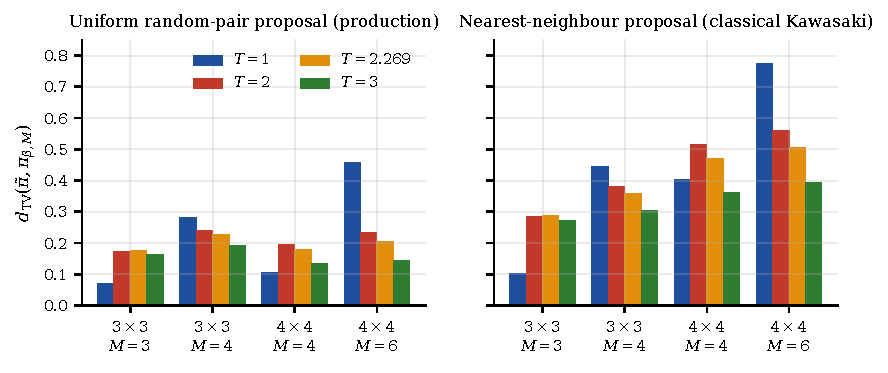
\includegraphics[width=\linewidth]{figures/fig_exact_tv.pdf}
\caption{\textbf{Total-variation distance of the stationary law of the kernel without the adjacency term to the canonical law} on small tori (exact; E2). The corrected kernel has $d_{\TV}<\EtwoMaxTVcorrect$ in all cases (not shown). Left: production random-pair proposal; right: nearest-neighbour proposal.}
\label{fig:exact}
\end{figure}

\subsection{How far does a local error travel?}
\label{sec:results-impact}
At production sizes the question is how much of the one-step perturbation survives in equilibrium averages.

\paragraph{Footprint.} The empirical fraction of adjacent proposals matches $4/N^2$ (\cref{tab:adj}, appendix); at $N=100$ it is $\EthreeAdjHundred$ against $0.0004$, and the fraction of \emph{effective} (unlike-spin) proposals that are adjacent is at most $\EthreeAdjDiffMaxHundred$. The experiment kernels coincide draw-for-draw with the package kernel (equivalence: \EthreeEquivOK).

\paragraph{Equilibrium averages.} \Cref{fig:impact,tab:impact-fit,tab:impact} report E4 (the full table is in the appendix). At $N=8$ and $N=16$ the missing term shifts the mean energy per site upwards by $5.5$--$6.3\%$ and $1.0$--$2.2\%$ respectively (all six comparisons have $|z|\ge5.5$). The ratio of the two effects at $T=1.5$ is $\EfourSmallRatio$, close to the factor $4$ expected if the effect scales with the footprint $N^{-2}$. At $N\ge32$ we cannot distinguish the shift from zero: $\EfourCountLargeSig$ of $\EfourCountLarge$ comparisons has $|z|>1.96$, about what nine comparisons produce under the null. A weighted fit $\Delta\langle e\rangle=c/N^2$ over all five sizes (\cref{tab:impact-fit}) gives $c=4.4\pm0.2$, $3.7\pm0.1$ and $2.35\pm0.10$ at $T=1.5$, $\Tc$ and $3$, with fit $p$-values $0.22$, $0.02$ and $0.44$. The $N^{-2}$ law describes the data at two temperatures and is in moderate tension with them at $T=\Tc$. Extrapolating, the predicted shift at $N=32$ is about $\EfourPredThirtyTwo$ against a standard error of $\EfourSeThirtyTwo$ per comparison, below our resolution.

What this establishes is limited. The kernel without the adjacency term is wrong, its effect is measurable and large at small $N$, and it scales as the footprint suggests. We do not claim it changes macroscopic results at $N\ge32$ under random-pair proposals; our replication has too little power to say. We did not analyse its effect on variances or higher moments, which are what the variance-peak estimator uses.

\begin{figure}[t]
\centering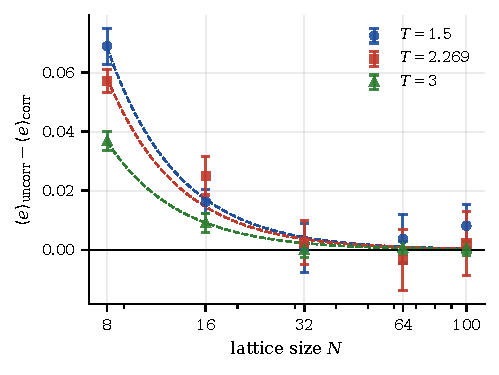
\includegraphics[width=0.62\linewidth]{figures/fig_adjacency_impact.pdf}
\caption{\textbf{Effect of omitting the adjacency term on the mean energy per site} ($f=1/2$; E4). Points: difference of replicate means with $95\%$ intervals ($1.96$ Welch standard errors); dashed: weighted fit $c/N^2$. Vertical axis is symmetric-log.}
\label{fig:impact}
\end{figure}


\begin{table}[t]
\centering\small
\caption{E4: weighted fits $\Delta\langle e\rangle=c/N^2$ over $N\in\{8,16,32,64,100\}$. $\chi^2$ (degrees of freedom) and $p$-value of the fit; $\chi^2_0$ and $p_0$ for the null $c=0$ (5 d.o.f.).}
\label{tab:impact-fit}
\begin{tabular}{@{}cccccrc@{}}
\toprule
$T$ & $c$ & s.e. & $\chi^2$ (d.o.f.) & $p$ & $\chi^2_0$ & $p_0$\\
\midrule
1.5 & 4.38 & 0.19 & 5.7 (4) & 0.22 & 565 & $<10^{-6}$ \\
2.269 & 3.73 & 0.13 & 11.2 (4) & 0.02 & 880 & $<10^{-6}$ \\
3 & 2.35 & 0.10 & 3.7 (4) & 0.44 & 521 & $<10^{-6}$\\
\bottomrule
\end{tabular}
\end{table}

\section{Results II: Does the Variance Peak Locate the Transition?}
\label{sec:results-demix}
With the sampler established, we compare the variance-peak estimate with the exact coexistence temperature, first for the single-seed protocol and then with replication.

\subsection{Single-seed and replicated estimates against the exact binodal}
\paragraph{Original single-seed protocol.} The single-seed protocol (E6: $N=100$, one seed per composition, a $20$-point grid on $[1.5,3.0]$) gives the estimates in \cref{tab:repo}. Against the exact binodal they deviate by between $\EsixMinDev$ and $\EsixMaxDev$ (maximum absolute deviation $\EsixMaxAbsDev$), the largest estimate is $\EsixMaxOver$---above $\Tc=\EbHalf$, the highest temperature at which the binodal exists---and the estimates at $f=0.05$ and $f=0.95$, which must coincide by the symmetry of \cref{def:binodal}, differ by $\EsixAsym$. Single-run noise of the size measured below produces features like these. The values lie within $\EsixZMax$ replicate standard deviations of the replicate means at $N=100$ (E5), so a single-seed curve is not evidence for or against any shape of the composition dependence.

\begin{table}[t]
\centering\small
\caption{Estimates of the single-seed protocol (E6; $N=100$, grid step $0.079$) against the exact binodal ($J=1$).}
\label{tab:repo}
\begin{tabular}{@{}cccc@{}}
\toprule
$f$ & $\Tb(f)$ exact & $\hat T^V$ (single seed) & deviation\\
\midrule
0.05 & 2.032 & 1.816 & -0.216 \\
0.10 & 2.188 & 1.974 & -0.214 \\
0.20 & 2.261 & 2.289 & +0.028 \\
0.30 & 2.269 & 2.447 & +0.178 \\
0.40 & 2.269 & 2.447 & +0.178 \\
0.60 & 2.269 & 2.289 & +0.020 \\
0.80 & 2.261 & 2.053 & -0.209 \\
0.95 & 2.032 & 1.579 & -0.453\\
\bottomrule
\end{tabular}
\end{table}

\paragraph{Replicated protocol.} \Cref{fig:demix,tab:demix} report E5 ($\EfiveR$ replicates per cell, all other protocol parameters unchanged). We apply the criteria fixed in \cref{sec:thermo}.
\begin{enumerate}[label=(\roman*),leftmargin=2em]
\item \emph{Single-run noise is large.} The standard deviation of $\hat T^V$ over replicates ranges from $\EfiveSdMin$ to $\EfiveSdMax$ across the $27$ cells, i.e.\ from $2$ to $6$ grid steps.
\item \emph{Central compositions ($0.2\le f\le0.8$).} The bootstrap interval of the replicate-mean peak contains $\Tb(f)$ in $\EfiveCentralIn$ of $\EfiveCentralTot$ cells, but the intervals are wide (widths $\EfiveCIWidthMin$--$\EfiveCIWidthMax$), so the test has little power to distinguish $\Tb(f)$ from values several tenths away. The single-run mean differs from $\Tb$ by more than two standard errors in $\EfiveCenZGtTwo$ of $\EfiveCenTot$ cells (maximum $|z|=\EfiveCenZMax$), with both signs. So the estimator is not unbiased for $\Tb(f)$ in the central range either, but its error there is at most $\EfiveCenBiasMax$, a few grid steps.
\item \emph{Dilute compositions ($f\in\{0.05,0.10,0.95\}$).} Here the estimator is biased \emph{low}: the single-run mean lies between $\EfiveExtBiasMin$ and $\EfiveExtBiasMax$ from $\Tb(f)$, with $|z|\ge\EfiveExtZMin$ in all $9$ cells, and the bootstrap interval contains $\Tb(f)$ in $\EfiveExtremeIn$ of $\EfiveExtremeTot$ cells. At $f=0.05$ the single-run means are $\EfiveMeanAtFiveHundredthXXXII$, $\EfiveMeanAtFiveHundredthLXIV$, $\EfiveMeanAtFiveHundredthC$ for $N=32,64,100$ against $\Tb=\EfiveTbAtFiveHundredth$: over this range of sizes the offset shows no detectable decrease with $N$.
\item \emph{Symmetry.} The estimator should be invariant under $f\leftrightarrow1-f$; \cref{tab:sym} shows differences between $\EfiveSymMin$ and $\EfiveSymMax$ at $N=100$, to be compared with a standard error of about $0.05$ for each entry.
\item \emph{Choice of functional.} The maximiser of the specific heat $\hat T^C$ lies systematically below $\hat T^V$ in the central range (\cref{tab:demix}, last column) and its bootstrap interval contains $\Tb$ in $\EfiveCentralInC$ of $\EfiveCentralTot$ central and $\EfiveExtremeInC$ of $\EfiveExtremeTot$ dilute cells.
\end{enumerate}
The replicated data support the qualitative shape ``roughly flat near $\Tc$ over the central range, lower at dilute compositions'', which is also the shape of $\Tb(f)$. They do not support the claim that the variance peak recovers the binodal quantitatively. At dilute compositions it is statistically distinguishable from $\Tb(f)$. In the central range, its resolution of a few grid steps is larger than the whole composition dependence of $\Tb$, which varies by only $\EbDevTwoTenths$ ($\EbRelTwoTenths\%$) between $f=0.2$ and $f=0.5$ and by $\EbDevThreeTenths$ between $f=0.3$ and $f=0.5$. Differences between central compositions in single-run estimates, such as the peak at $f=0.4$ in the single-seed curve, are noise.

\begin{figure}[t]
\centering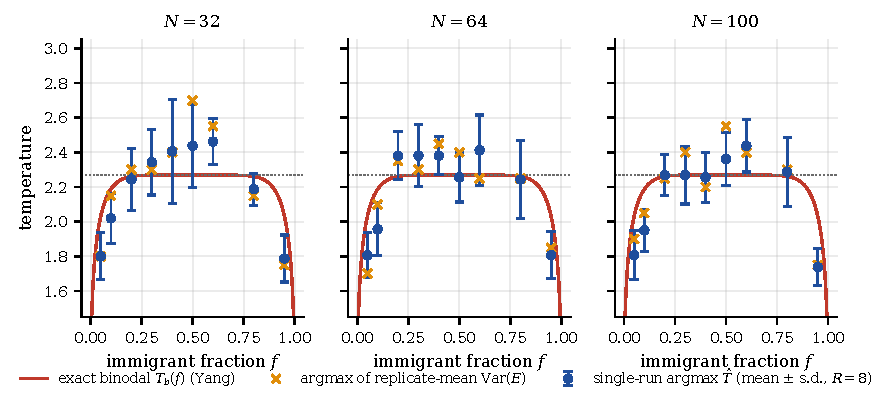
\includegraphics[width=\linewidth]{figures/fig_demixing.pdf}
\caption{\textbf{Variance-peak temperature against the exact coexistence curve} (E5). Blue: mean $\pm$ standard deviation over $\EfiveR$ replicates of the single-run estimator $\hat T^V$ (the original protocol on a grid of step $\EfiveGridStep$); orange crosses: maximiser of the replicate-mean $\Var(E)$; red: exact binodal $\Tb(f)$ (\cref{def:binodal}); dotted: $\Tc$.}
\label{fig:demix}
\end{figure}

\begin{figure}[t]
\centering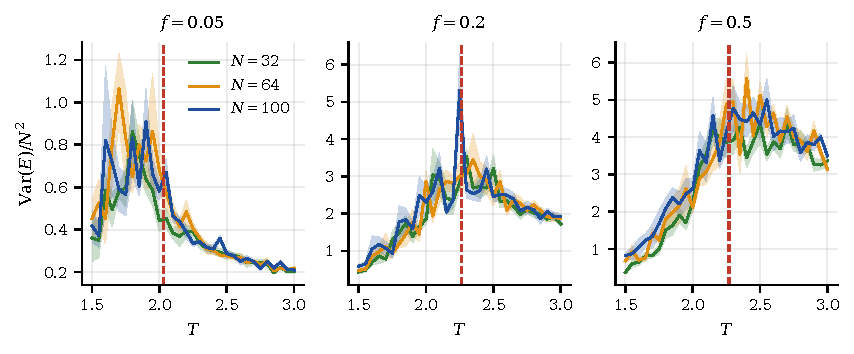
\includegraphics[width=\linewidth]{figures/fig_variance_curves.pdf}
\caption{\textbf{Replicate-mean energy variance per site} for three compositions and three sizes (E5; bands: $\pm1$ s.e.\ over $\EfiveR$ replicates). Dashed red: $\Tb(f)$. The curves are broad and noisy relative to the composition dependence of $\Tb$.}
\label{fig:curves}
\end{figure}

\begin{table}[t]
\centering\small
\caption{Symmetry check of the single-run estimator, $N=100$ (E5): mean of $\hat T^V$ over $\EfiveR$ replicates at $f$ and $1-f$.}
\label{tab:sym}
\begin{tabular}{@{}ccccc@{}}
\toprule
$f$ & $1-f$ & $\langle\hat T^V\rangle_f$ & $\langle\hat T^V\rangle_{1-f}$ & difference\\
\midrule
0.05 & 0.95 & 1.806 & 1.738 & 0.069 \\
0.20 & 0.80 & 2.269 & 2.287 & 0.019 \\
0.40 & 0.60 & 2.256 & 2.438 & 0.181\\
\bottomrule
\end{tabular}
\end{table}

\subsection{Is the sampling window long enough? Equilibration and an equilibrium reference}\label{sec:results-equil}
The protocol discards $\EfiveBurn$ sweeps and samples $\EfiveSample$ (\cref{sec:protocol}), and the estimator uses the variance of the energy in that window. Two diagnostics ask whether that window is adequate, and whether any inadequacy explains the dilute offset.

\paragraph{E9a: single long traces.} For $\EnineaCases$ cells ($N\in\{64,100\}$, one trace each, $\EnineaTotalSweeps$ sweeps from a random start; seed fixed) we compare the sampling window with late windows of the same length and with the long-run variance. \Cref{tab:E9a} lists the offset of the protocol-window mean from the late mean in units of the long-run standard deviation, and the ratio of the protocol-window variance to the long-run variance. The ratio ranges from $\EnineaRatioMin$ to $\EnineaRatioMax$ (median $\EnineaRatioMedian$); in $\EnineaBelowHalf$ of $\EnineaCases$ cells it is below $1/2$, and the mean offset exceeds one standard deviation in $\EnineaOffGtOne$ cells (maximum $\EnineaOffMax$). The window is therefore not equilibrated in every cell, notably at low temperature and dilute composition, and its variance is on the whole biased low and noisy. Each cell has a single trace, so the table documents the effect without estimating its distribution.

\begin{table}[t]
\centering\small
\caption{E9a. Protocol window (sweeps 500--800) versus late windows (sweeps 20\,000--40\,000) of one trace per cell. Offset: protocol mean minus late mean, in units of the long-run standard deviation of $E$. $V_{\rm prot}$, $V_{\rm late}$: variance of $E$ in the two windows; the last column is their ratio.}\label{tab:E9a}
\begin{tabular}{rrrrrrr}
\toprule
$N$ & $f$ & $T$ & offset & $V_{\rm prot}$ & $V_{\rm late}$ & ratio\\
\midrule
64 & 0.05 & 1.8 & +2.1 & 1480 & 8449 & 0.18 \\
64 & 0.05 & 2 & +0.3 & 1601 & 2890 & 0.55 \\
64 & 0.05 & 2.2 & -0.0 & 1708 & 1805 & 0.95 \\
64 & 0.20 & 2 & +1.3 & 9158 & 12395 & 0.74 \\
64 & 0.20 & 2.2 & -0.1 & 10308 & 21325 & 0.48 \\
64 & 0.20 & 2.4 & -0.1 & 18921 & 13995 & 1.35 \\
64 & 0.50 & 2.2 & +0.6 & 7019 & 24157 & 0.29 \\
64 & 0.50 & 2.4 & +0.4 & 23346 & 25216 & 0.93 \\
64 & 0.50 & 2.6 & +0.2 & 12048 & 18754 & 0.64 \\
100 & 0.05 & 1.8 & +2.3 & 4353 & 17198 & 0.25 \\
100 & 0.05 & 2 & +0.2 & 4910 & 8747 & 0.56\\
\bottomrule
\end{tabular}
\end{table}

\paragraph{E9b: equilibrium reference.} To separate the effect of the short window from the finite-size behaviour of the estimator, we re-ran six $(N,f)$ systems on the temperature grid $1.5\le T\le2.8$ in steps of $0.05$ with $10\,000$ burn-in sweeps and $50\,000$ sampling sweeps, using $3$ replicates for $N=32$ and $2$ for $N=64$ ($\EninebRuns$ runs in total). The integrated autocorrelation time of the energy (Sokal windowing) has median $\EninebTauMedian$ sweeps over all runs and maximum $\EninebTauMax$ sweeps; the maximum is more than ten times the 300-sweep window, so the window is shorter than $\tau_{\rm int}$ in the worst cells.

\Cref{tab:E9b} and \cref{fig:equilibrium} report the temperature of the peak of the replicate-mean variance under the long run, the range of the per-replicate peaks, the peak of the specific heat $\mathrm{Var}(E)/(N^2T^2)$, and the corresponding peak of the original protocol of E5, next to the exact binodal $\Tb(f)$.

\begin{table}[t]
\centering\small
\caption{E9b. Variance-peak temperature under the long equilibrium protocol versus the exact binodal. $\Tb$: exact binodal; $\hat T_{\rm eq}$: peak of the replicate-mean $\mathrm{Var}(E)$; range: smallest--largest per-replicate peak; $\hat T_C$: peak of the replicate-mean specific heat; $\hat T_{\rm prot}$: peak of the mean variance under the 300-sweep protocol (E5); $\tau$: mean $\tau_{\rm int}$ (sweeps) at $\hat T_{\rm eq}$. Grid step $0.05$.}\label{tab:E9b}
\begin{tabular}{rrrrrrrr}
\toprule
$N$ & $f$ & $\Tb$ & $\hat T_{\rm eq}$ & range & $\hat T_C$ & $\hat T_{\rm prot}$ & $\tau$\\
\midrule
32 & 0.05 & 2.032 & 1.75 & 1.75--1.75 & 1.65 & 1.80 & 80 \\
32 & 0.10 & 2.188 & 2.00 & 1.95--2.00 & 1.90 & 2.15 & 59 \\
32 & 0.20 & 2.261 & 2.15 & 2.15--2.20 & 2.15 & 2.30 & 48 \\
32 & 0.50 & 2.269 & 2.40 & 2.35--2.40 & 2.20 & 2.70 & 21 \\
64 & 0.05 & 2.032 & 1.85 & 1.85--1.85 & 1.85 & 1.70 & 258 \\
64 & 0.50 & 2.269 & 2.30 & 2.25--2.30 & 2.30 & 2.40 & 87\\
\bottomrule
\end{tabular}
\end{table}

\begin{figure}[t]
\centering
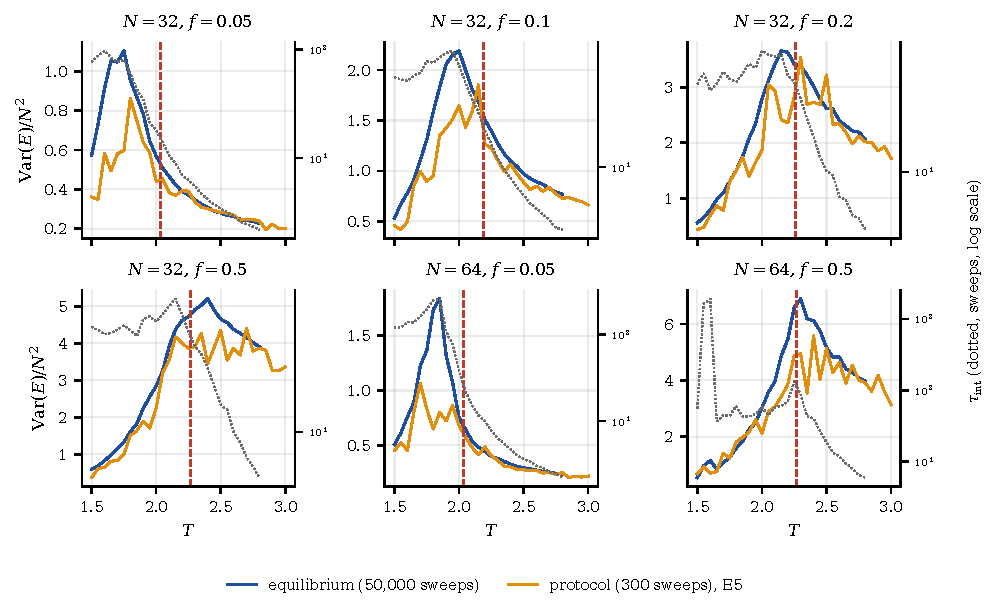
\includegraphics[width=\linewidth]{figures/fig_equilibrium.pdf}
\caption{E9b. $\mathrm{Var}(E)/N^2$ versus $T$ under the long equilibrium protocol (blue) and the 300-sweep protocol of E5 (orange); dashed vertical line: exact binodal; dotted: $\tau_{\rm int}$ on a logarithmic axis (right).}\label{fig:equilibrium}
\end{figure}

We read \cref{tab:E9b} with its limits in mind: a $0.05$ grid and two or three replicates.
(i) The protocol and equilibrium peaks differ by at most $0.30$ in $T$ (largest at $N=32$, $f=0.5$). The window effect seen in E9a moves the estimate by a few grid steps; it does not explain the dilute offsets of \cref{sec:results-demix}.
(ii) For $f=0.05$ the equilibrium peak lies below $\Tb$ ($1.75$ versus $2.032$ at $N=32$, $1.85$ versus $2.032$ at $N=64$); at $f=0.10$ and $0.20$ at $N=32$ it lies $0.19$ and $0.11$ below. The gap at $f=0.05$ is smaller at $N=64$ than at $N=32$, but the $N=64$ peaks come from two replicates on a coarse grid, so all we can say is that the data do not contradict a decreasing offset. The direction agrees with finite-size droplet formation \citep{binder1987,biskup2002}; we did not test the scaling.
(iii) At $f=0.5$ the equilibrium peak lies above the critical temperature ($2.40$ at $N=32$, $2.30$ at $N=64$ versus $\Tc=2.269$), consistent with a finite-size shift towards $\Tc$ from above as $N$ grows.
The variance peak is a finite-size quantity. Its location depends on $N$ and, in part, on the window length, and it should not be identified with $\Tb$ without a finite-size analysis.

\section{Discussion}\label{sec:discussion}
\paragraph{Two ways a simulation can mislead.} The study separates two failure modes. The first is in the sampler. A kernel that looks right can lack detailed balance, and we showed exactly how: dropping the adjacency term multiplies the flux by $e^{\pm4\beta J}$ on adjacent exchanges (\cref{prop:flux}), and on tori we can solve this moves the stationary law by $\EtwoPairMin$--$\EtwoNNMax$ in total variation. The correct kernel has the canonical law as its unique stationary distribution (\cref{thm:correct}). At large $N$ under random-pair proposals the local error shrinks like $N^{-2}$, but we could not conclude from this that equilibrium averages are accurate, and measurement bore this out only partly: the effect is clear at $N=8,16$ and invisible at $N\ge32$ with our replication. A one-step bound is not a bound on the stationary law.

The second failure is in the question. Once the sampler is right, the variance peak is still not the coexistence temperature. In the central range, the exact curve varies by $\EbDevTwoTenths$ ($\EbRelTwoTenths\%$) while the single-run standard deviation is $\EfiveSdMin$--$\EfiveSdMax$, so composition dependence read off one simulated curve is noise. At dilute compositions the peak sits $0.17$--$0.29$ below the exact curve, and a long equilibrium reference leaves it there. The 300-sweep window does distort the variance, since $\tau_{\rm int}$ reaches $\EninebTauMax$ sweeps in the worst cells, but it does not by itself explain the offset.

\paragraph{Practical consequences.} For exchange moves, test the acceptance rule against brute-force energy differences on all local configurations; it takes seconds. For transition temperatures, report replicate-based uncertainty, compare with an exact reference when one exists, and use a sampling window well beyond the autocorrelation time. For this model, treat apparent composition dependence of a variance peak inside $0.2\le f\le0.8$ as noise at the resolutions we used.

\paragraph{What this study does not establish.} We studied one model: the two-dimensional square-lattice Ising lattice gas with $J=1$, periodic boundaries and uniform random-pair proposals, at $N\le100$. The proposals are non-local, so we say nothing about relaxation or coarsening kinetics. The exact stationary laws are limited to tori of at most $8008$ states and therefore to footprints far larger than at production sizes. In the impact study (E4) we examined only the mean energy at $f=1/2$, with at most $20$ replicates at $N=100$; the null results at $N\ge32$ reflect limited power, not demonstrated absence of an effect, and the $N^{-2}$ law is in moderate tension with the $T=\Tc$ data ($p=0.02$). The variance-peak study used $R=\EfiveR$ replicates, a grid step of $\EfiveGridStep$, the $\EfiveBurn+\EfiveSample$-sweep protocol and three sizes, so the dependence of the dilute offset on $N$ is resolved only as ``no detectable decrease''. The equilibrium reference used at most three replicates at $N\le64$ and did not examine the scaling of the offset with $N$. Our argument that the specific heat has a finite jump at the binodal in the thermodynamic limit is a standard thermodynamic argument that we neither derived nor tested. We compared the variance and specific-heat peaks only, not other estimators, and we do not interpret the model sociologically.

\paragraph{Conclusion.} For a Kawasaki--Ising model of segregation we derived the exact exchange energy, proved that the resulting kernel samples the canonical law, and measured how much omitting the adjacency term would matter at small and large sizes. We then compared the variance-peak temperature with the exact fixed-composition coexistence curve using replicated runs and a long equilibrium reference. The peak is too noisy to resolve the composition dependence of the exact curve in the central range and falls below it at dilute compositions, for reasons we attribute neither to the sampler nor only to the sampling window. A plausible-looking figure checks neither one. Both the kernel and the estimator have to be tested against something exact.


\section*{Code and data availability}
The code, the raw outputs of every experiment and the scripts that generate each figure, table and number in this paper are in the repository accompanying it (\cref{app:repro}).

\bibliographystyle{plainnat}
\bibliography{references}
\appendix
\section{Complete Exact-Chain Results}
\label{app:exact}
\begin{table}[h]
\centering\small
\caption{All exact stationary-law results (E2) at the four temperatures studied; columns as in \cref{tab:exact}. The correct kernel is at the solver precision in every row.}
\label{tab:exact-full}
\begin{tabular}{@{}cccc c cc cc@{}}
\toprule
 &  &  &  & correct & \multicolumn{2}{c}{uncorrected, pair} & \multicolumn{2}{c}{uncorrected, NN}\\
\cmidrule(lr){5-5}\cmidrule(lr){6-7}\cmidrule(lr){8-9}
torus & $M$ & $|\Omega|$ & $T$ & $d_{\TV}$ & $d_{\TV}$ & $\Delta\langle E\rangle$ & $d_{\TV}$ & $\Delta\langle E\rangle$\\
\midrule
$3\times3$ & 3 & 84 & 1 & $4\times10^{-14}$ & 0.070 & +0.543 & 0.102 & +0.833 \\
$3\times3$ & 3 & 84 & 2 & $8\times10^{-15}$ & 0.174 & +1.294 & 0.285 & +1.960 \\
$3\times3$ & 3 & 84 & 2.269 & $1\times10^{-14}$ & 0.177 & +1.266 & 0.290 & +1.933 \\
$3\times3$ & 3 & 84 & 3 & $5\times10^{-15}$ & 0.164 & +1.101 & 0.273 & +1.726 \\
$3\times3$ & 4 & 126 & 1 & $3\times10^{-15}$ & 0.282 & +1.454 & 0.444 & +2.543 \\
$3\times3$ & 4 & 126 & 2 & $2\times10^{-15}$ & 0.241 & +1.371 & 0.380 & +2.345 \\
$3\times3$ & 4 & 126 & 2.269 & $4\times10^{-15}$ & 0.227 & +1.324 & 0.359 & +2.259 \\
$3\times3$ & 4 & 126 & 3 & $3\times10^{-15}$ & 0.191 & +1.176 & 0.306 & +2.008 \\
$4\times4$ & 4 & 1\,820 & 1 & $1\times10^{-13}$ & 0.106 & +0.882 & 0.402 & +3.804 \\
$4\times4$ & 4 & 1\,820 & 2 & $3\times10^{-14}$ & 0.197 & +1.450 & 0.514 & +4.346 \\
$4\times4$ & 4 & 1\,820 & 2.269 & $7\times10^{-14}$ & 0.180 & +1.338 & 0.471 & +3.999 \\
$4\times4$ & 4 & 1\,820 & 3 & $2\times10^{-14}$ & 0.134 & +1.049 & 0.361 & +3.203 \\
$4\times4$ & 6 & 8\,008 & 1 & $1\times10^{-13}$ & 0.458 & +2.780 & 0.774 & +7.819 \\
$4\times4$ & 6 & 8\,008 & 2 & $5\times10^{-14}$ & 0.234 & +2.000 & 0.560 & +5.980 \\
$4\times4$ & 6 & 8\,008 & 2.269 & $9\times10^{-14}$ & 0.206 & +1.812 & 0.507 & +5.503 \\
$4\times4$ & 6 & 8\,008 & 3 & $3\times10^{-14}$ & 0.145 & +1.406 & 0.393 & +4.439\\
\bottomrule
\end{tabular}
\end{table}

\section{Complete Variance-Peak Results}
\label{app:demix}
\begin{table}[h]
\centering\footnotesize
\caption{All cells of E5. $\Tb$: exact binodal; $\langle\hat T^V\rangle$ and s.d.: mean and standard deviation of the single-run estimator over $\EfiveR$ replicates; $z=(\langle\hat T^V\rangle-\Tb)/(\mathrm{s.d.}/\sqrt{R})$; $\bar T^V$ and CI: maximiser of the replicate-mean $\hat V$ and its $95\%$ bootstrap percentile interval ($4000$ resamples); ``in'': whether the interval contains $\Tb$; $\bar T^C$: maximiser of the replicate-mean specific heat. Grid step $\EfiveGridStep$.}
\label{tab:demix}
\setlength{\tabcolsep}{4pt}
\begin{tabular}{@{}rcccccccccc@{}}
\toprule
$N$ & $f$ & $\Tb$ & $\langle\hat T^V\rangle$ & s.d. & $z$ & $\bar T^V$ & CI & in & $\bar T^C$\\
\midrule
32 & 0.05 & 2.032 & 1.800 & 0.136 & -4.8 & 1.80 & [1.80, 1.85] & no & 1.80 \\
32 & 0.10 & 2.188 & 2.019 & 0.146 & -3.3 & 2.15 & [1.90, 2.15] & no & 2.00 \\
32 & 0.20 & 2.261 & 2.244 & 0.178 & -0.3 & 2.30 & [2.05, 2.50] & yes & 2.05 \\
32 & 0.30 & 2.269 & 2.344 & 0.190 & +1.1 & 2.30 & [2.15, 2.55] & yes & 2.30 \\
32 & 0.40 & 2.269 & 2.406 & 0.299 & +1.3 & 2.40 & [2.25, 2.60] & yes & 2.25 \\
32 & 0.50 & 2.269 & 2.438 & 0.240 & +2.0 & 2.70 & [2.15, 2.70] & yes & 2.15 \\
32 & 0.60 & 2.269 & 2.462 & 0.133 & +4.1 & 2.55 & [2.25, 2.55] & yes & 2.10 \\
32 & 0.80 & 2.261 & 2.188 & 0.092 & -2.3 & 2.15 & [2.15, 2.25] & no & 2.15 \\
32 & 0.95 & 2.032 & 1.788 & 0.136 & -5.1 & 1.75 & [1.65, 1.90] & no & 1.65 \\
\midrule
64 & 0.05 & 2.032 & 1.806 & 0.129 & -4.9 & 1.70 & [1.65, 1.95] & no & 1.70 \\
64 & 0.10 & 2.188 & 1.956 & 0.152 & -4.3 & 2.10 & [1.75, 2.10] & no & 1.80 \\
64 & 0.20 & 2.261 & 2.381 & 0.139 & +2.4 & 2.35 & [2.15, 2.55] & yes & 2.00 \\
64 & 0.30 & 2.269 & 2.381 & 0.179 & +1.8 & 2.30 & [2.20, 2.65] & yes & 2.30 \\
64 & 0.40 & 2.269 & 2.381 & 0.110 & +2.9 & 2.45 & [2.25, 2.45] & yes & 2.25 \\
64 & 0.50 & 2.269 & 2.256 & 0.143 & -0.3 & 2.40 & [2.25, 2.50] & yes & 2.40 \\
64 & 0.60 & 2.269 & 2.413 & 0.203 & +2.0 & 2.25 & [2.20, 2.60] & yes & 2.25 \\
64 & 0.80 & 2.261 & 2.244 & 0.224 & -0.2 & 2.25 & [1.80, 2.40] & yes & 2.10 \\
64 & 0.95 & 2.032 & 1.806 & 0.135 & -4.7 & 1.85 & [1.75, 1.90] & no & 1.85 \\
\midrule
100 & 0.05 & 2.032 & 1.806 & 0.143 & -4.5 & 1.90 & [1.60, 1.90] & no & 1.60 \\
100 & 0.10 & 2.188 & 1.950 & 0.122 & -5.5 & 2.05 & [1.70, 2.05] & no & 2.05 \\
100 & 0.20 & 2.261 & 2.269 & 0.119 & +0.2 & 2.25 & [2.25, 2.45] & yes & 2.25 \\
100 & 0.30 & 2.269 & 2.269 & 0.167 & -0.0 & 2.40 & [2.10, 2.50] & yes & 2.10 \\
100 & 0.40 & 2.269 & 2.256 & 0.145 & -0.3 & 2.20 & [2.10, 2.40] & yes & 2.20 \\
100 & 0.50 & 2.269 & 2.362 & 0.153 & +1.7 & 2.55 & [2.15, 2.55] & yes & 2.15 \\
100 & 0.60 & 2.269 & 2.438 & 0.151 & +3.2 & 2.40 & [2.30, 2.60] & no & 2.30 \\
100 & 0.80 & 2.261 & 2.287 & 0.198 & +0.4 & 2.30 & [2.15, 2.30] & yes & 2.15 \\
100 & 0.95 & 2.032 & 1.738 & 0.106 & -7.9 & 1.75 & [1.65, 1.90] & no & 1.75\\
\bottomrule
\end{tabular}
\end{table}

\section{Supporting Tables for the Sampler Checks}\label{app:sampler-tables}
\begin{table}[t]
\centering\small
\caption{Empirical proposal statistics of the corrected sampler ($f=0.2$; $300$ burn-in and $300$ measured sweeps, single run each; E3). ``adjacent'' is the fraction of all proposals with $x\sim y$; ``adj.\ among unlike'' the fraction of unlike-spin proposals that are adjacent.}
\label{tab:adj}
\begin{tabular}{@{}rcccc c@{}}
\toprule
$N$ & $T$ & adjacent & $4/N^2$ & adj.\ among unlike & acceptance among unlike\\
\midrule
20 & 1 & 0.00998 & 0.01000 & 0.00173 & 0.007 \\
20 & 2.269 & 0.00958 & 0.01000 & 0.00579 & 0.218 \\
20 & 3 & 0.00991 & 0.01000 & 0.00681 & 0.414 \\
40 & 1 & 0.00253 & 0.00250 & 0.00043 & 0.005 \\
40 & 2.269 & 0.00262 & 0.00250 & 0.00119 & 0.194 \\
40 & 3 & 0.00257 & 0.00250 & 0.00181 & 0.396 \\
100 & 1 & 0.00040 & 0.00040 & 0.00004 & 0.005 \\
100 & 2.269 & 0.00043 & 0.00040 & 0.00019 & 0.185 \\
100 & 3 & 0.00040 & 0.00040 & 0.00027 & 0.390\\
\bottomrule
\end{tabular}
\end{table}

\begin{table}[t]
\centering\small
\caption{E4: mean energy per site under the corrected and uncorrected rules ($f=1/2$). $R$ replicates per rule; $z$ is the difference divided by its Welch standard error.}
\label{tab:impact}
\begin{tabular}{@{}rcrccccc@{}}
\toprule
$N$ & $T$ & $R$ & $\langle e\rangle_{\rm corr}$ & $\langle e\rangle_{\rm uncorr}$ & difference & s.e. & $z$\\
\midrule
8 & 1.5 & 400 & -1.23992 & -1.17096 & +0.06897 & 0.00309 & +22.3 \\
8 & 2.269 & 400 & -0.91124 & -0.85395 & +0.05729 & 0.00200 & +28.7 \\
8 & 3 & 400 & -0.67223 & -0.63532 & +0.03692 & 0.00167 & +22.1 \\
16 & 1.5 & 200 & -1.57567 & -1.55937 & +0.01630 & 0.00208 & +7.8 \\
16 & 2.269 & 200 & -1.16087 & -1.13576 & +0.02511 & 0.00333 & +7.5 \\
16 & 3 & 200 & -0.78226 & -0.77317 & +0.00909 & 0.00165 & +5.5 \\
32 & 1.5 & 100 & -1.72008 & -1.71939 & +0.00069 & 0.00418 & +0.2 \\
32 & 2.269 & 100 & -1.28068 & -1.27816 & +0.00253 & 0.00377 & +0.7 \\
32 & 3 & 100 & -0.80736 & -0.80749 & -0.00013 & 0.00127 & -0.1 \\
64 & 1.5 & 40 & -1.77718 & -1.77344 & +0.00375 & 0.00417 & +0.9 \\
64 & 2.269 & 40 & -1.34102 & -1.34448 & -0.00346 & 0.00530 & -0.7 \\
64 & 3 & 40 & -0.81469 & -0.81398 & +0.00070 & 0.00117 & +0.6 \\
100 & 1.5 & 20 & -1.78753 & -1.77937 & +0.00816 & 0.00369 & +2.2 \\
100 & 2.269 & 20 & -1.35126 & -1.34907 & +0.00219 & 0.00559 & +0.4 \\
100 & 3 & 20 & -0.81604 & -0.81556 & +0.00048 & 0.00115 & +0.4\\
\bottomrule
\end{tabular}
\end{table}

\section{A Side Check: Translation Invariance of the Clustering Metric}\label{app:metric}
The kernel $P_\beta$ and the law $\pi_{\beta,M}$ are invariant under translations of the torus, so a summary of the state should be too. This check is separate from the main argument; we include it because the software reports a clustering summary. The clustering summary used in the accompanying software is the mean pairwise distance of immigrants. With $d_{\Lam}(x,y)=\big(\sum_{i=1}^{2}\min\{|x_i-y_i|,N-|x_i-y_i|\}^2\big)^{1/2}$ the toroidal (minimum-image) metric and $\mathcal I(\sigma)=\{x:\sigma_x=+1\}$,
\[
D_{\mathrm{per}}(\sigma)=\binom{M}{2}^{-1}\!\!\!\sum_{\{x,y\}\subset\mathcal I(\sigma)}\!\!\! d_{\Lam}(x,y),
\]
while $D_{\mathrm{euc}}$ uses instead the Euclidean distance of the integer coordinates in $\{0,\dots,N-1\}^2$.
\begin{proposition}[Translation invariance]\label{prop:metric}
$D_{\mathrm{per}}(\theta_a\sigma)=D_{\mathrm{per}}(\sigma)$ for all $a\in\Lam$, whereas $D_{\mathrm{euc}}$ is not translation invariant: for $M=2$ with immigrants at $(0,0)$ and $(N-1,0)$ one has $D_{\mathrm{euc}}=N-1$, but after translating by $(1,0)$ one has $D_{\mathrm{euc}}=1$.
\end{proposition}
\begin{proof}
$d_{\Lam}(x+a,y+a)=d_{\Lam}(x,y)$ because the minimum-image differences are unchanged; the counterexample is a direct computation.
\end{proof}

In E8 the periodic mean immigrant distance $D_{\mathrm{per}}$ of $25$ random translates of one equilibrated configuration ($N=100$, $f=0.2$, $T=1$, $3000$ sweeps) varies by $\EeightPerSpread$ (floating-point level; value $\EeightPer$). The non-periodic $D_{\mathrm{euc}}$ ranges from $\EeightNonMin$ to $\EeightNonMax$, a spread of $\EeightNonRel\%$ of its mean, although all $25$ configurations are the same physical state (\cref{prop:metric}). Values and trends of $D_{\mathrm{euc}}$ across runs or compositions therefore cannot be read as properties of the model.

\section{Reproducibility}
\label{app:repro}
All experiments are scripts in \texttt{experiments/}; each writes its raw output to \texttt{results/paper/}, and \texttt{experiments/make\_paper\_assets.py} regenerates every figure and table of this paper (directory \texttt{paper/generated} and \texttt{paper/figures}). With Python $\ge3.10$, \texttt{numpy}, \texttt{scipy}, \texttt{matplotlib}, \texttt{numba} installed, the sequence is
\begin{center}\small\ttfamily
python experiments/exp\_exact\_local.py;\ python experiments/exp\_exact\_chain.py;\\
python experiments/exp\_verify\_dynamics.py;\ python experiments/exp\_adjacency\_impact.py;\\
python experiments/exp\_demixing.py;\ python experiments/exp\_single\_seed.py;\\
python experiments/exp\_metric\_invariance.py;\ python experiments/exp\_equilibration.py;\\
python experiments/exp\_equilibrium\_variance.py;\ python experiments/make\_paper\_assets.py
\end{center}
Wall-clock times on the two-core machine of \cref{sec:protocol}: E5 $\approx 22$ minutes, E9b $\approx$ 22 minutes, the remaining experiments a few minutes each. Seeds are derived by \texttt{SeedSequence} from the cell coordinates (\cref{sec:protocol}), so reruns on the same software versions reproduce the stored outputs.

\end{document}
